\documentclass[a4paper,10pt]{article}

\usepackage[french]{babel}
\usepackage[utf8]{inputenc}
\usepackage[left=2.5cm,top=2cm,right=2.5cm,nohead,nofoot]{geometry}
\usepackage{url}
\usepackage{graphicx}
\usepackage{hyperref}
\usepackage{listings}
\usepackage{amsmath}
\usepackage{color}

\lstset{
  language=SQL,
  basicstyle=\ttfamily\footnotesize,        % the size of the fonts that are used for the code
  breakatwhitespace=false,         % sets if automatic breaks should only happen at whitespace
  breaklines=true,                 % sets automatic line breaking
  commentstyle=\color{cyan},    % comment style
  keepspaces=true,                 % keeps spaces in text, useful for keeping indentation of code (possibly needs columns=flexible)
  keywordstyle=\color{blue},       % keyword style
  numbers=left,                    % where to put the line-numbers; possible values are (none, left, right)
  numbersep=5pt,                   % how far the line-numbers are from the code
  numberstyle=\tiny\color{blue}, % the style that is used for the line-numbers
  rulecolor=\color{black},         % if not set, the frame-color may be changed on line-breaks within not-black text (e.g. comments (green here))
  showstringspaces=false,          % underline spaces within strings only
  showtabs=false,                  % show tabs within strings adding particular underscores
  stepnumber=5,                    % the step between two line-numbers. If it's 1, each line will be numbered
  stringstyle=\color{red},     % string literal style
  tabsize=2,                       % sets default tabsize to 2 spaces
}


\linespread{1.1}



\begin{document}

\begin{titlepage}
\begin{center}
\textbf{\textsc{UNIVERSIT\'E LIBRE DE BRUXELLES}}\\
%\textbf{\textsc{Faculté des Sciences}}\\
%\textbf{\textsc{Département d'Informatique}}
\vfill{}\vfill{}
\begin{center}{\Huge Rapport : Villo !}\end{center}{\Huge \par}
\begin{center}{\large Pierre Gérard, Titouan Christophe}\end{center}{\Huge \par}
\vfill{}\vfill{} \vfill{}
\begin{flushleft}{\large \textbf{INFO-H-303 Base de données}}\hfill{Esteban Zimányi, Michaël Waumans}\end{flushleft}{\large\par}
\vfill{}\vfill{}\enlargethispage{3cm}
\textbf{Année académique 2014~-~2015}
\end{center}
\end{titlepage}

%\begin{abstract}
%Ce rapport présente ...
%\end{abstract}


\tableofcontents

\pagebreak


\section{Diagramme entité association}
\subsection{Diagramme}
\begin{figure}[hbt]
  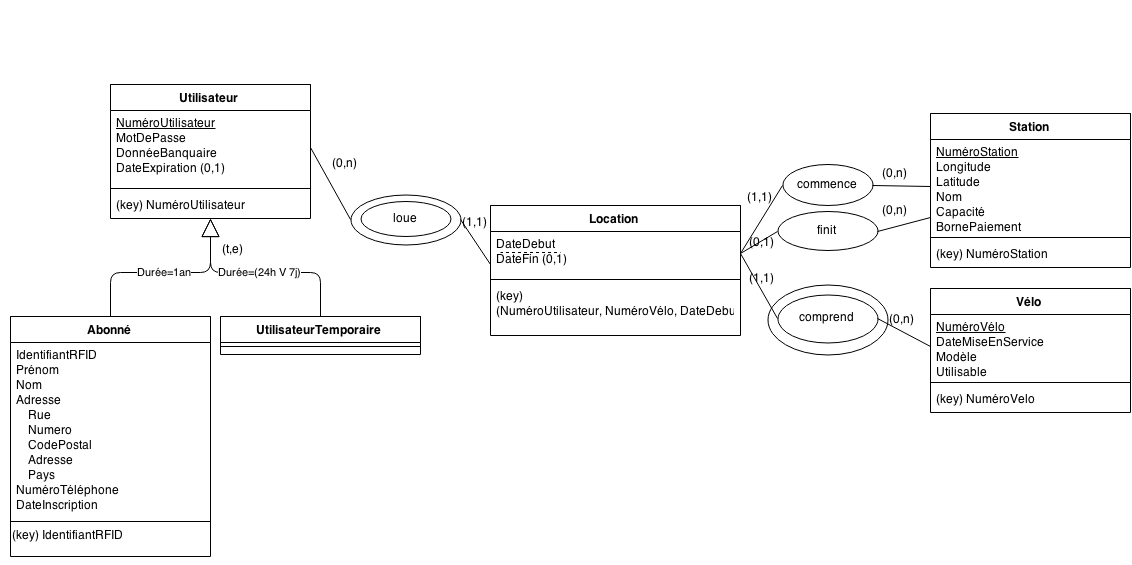
\includegraphics[scale=0.4]{dia/diagramme-entite-association.png}
  \caption{Diagramme entité association
}
\end{figure}
\subsection{Contraintes}
Les contraintes sont les suivantes :
\begin{itemize}
  \item La DateDebut d'une Location doit précéder la DateFin, 
  \item La DateMiseEnService d'un Vélo doit précéder la DateDebut de chacune de ses Locations,
  \item La DateExpiration d'un Utilisateur doit \^etre postérieure à la DateDebut de toutes ses Locations,
  \item Le couple (Longitude, Latitude) est unique,
  \item La DateExpiration d'un Utilisateur doit \^etre postérieure à la DateFin de toutes ses Locations,
  \item Un utilisateur qui a une date d'expiration non nul ne peut pas avoir plus d'une Location ayant une DateFin nul,
  \item Pour une Station, le nombre de vélo dont la dernière Location finit  dans cette station ne doit pas dépasser sa capacité,
  \item Un Vélo ne peut pas avoir de déplacement disjoints. C'est a dire que la Station de départ du trajet n doit \^etre similaire a la Station d'arrivé du trajet (n-1) pour n>1,
  \item Un Utilisateur ayant une DateExpiration non nul ne peut pas prendre un Vélo si Usable est faux.
\end{itemize}



\section{Modèle relationnel}
\subsection{Modèle}


\begin{description}
\item[] \textbf{Utilisateur}(\underline{NuméroUtilisateur}, MotDePasse, DonnéeBanquaire, \textit{DateExpiration})

\item[] \textbf{Abonné}(\underline{NuméroUtilisateur}, IdentifiantRFID, Nom, Rue, Numero, CodePostal, Adresse, Pays DateInscription, NuméroTélephone)
	\begin{description}
	\item[] Abonné.NuméroUtilisateur référence Utilisateur.NuméroUtilisateur
	\end{description}

\item[] \textbf{Location}(\underline{NuméroUtilisateur, NuméroVélo, DateDebut},\textit{DateFin}, NuméroStationDépart , NuméroStationFin) % par sur de la notation pour NuméroStationDépart ???
	\begin{description}
	\item[] Location.NuméroUtilisateur référence Utilisateur.NuméroUtilisateur
	\item[] Location.NuméroVélo référence Vélo.NuméroVélo
	\item[] Location.NuméroStationDépart référence Station.NuméroStation
	\item[] Location.NuméroStationFin référence Station.NuméroStation
	\item[] (\underline{NuméroUtilisateur, DateDebut}) est unique
	\item[] (\underline{NuméroVélo, DateDebut}) est unique
	\end{description}
	
\item[] \textbf{Station}(\underline{NuméroStation}, Longitude, Latitude, Nom, Capacité, BornePaiement)

\item[] \textbf{Vélo}(\underline{NuméroVélo}, DateMiseEnService, Modèle, Utilisable)

\end{description}

\subsection{Contraintes}

Les contraintes sont les suivantes :
\begin{itemize}
  \item Une Location a au plus une station d'arrivé,
  \item Une Location a une et une seule Station de départ,
  \item Une Location a un et un seul Utilisateur,
  \item Une Location a un et un seul Vélo,
  \item La DateDebut d'une Location doit précéder la DateFin, 
  \item La DateMiseEnService d'un Vélo doit précéder la DateDebut de chacune de ses Locations,
  \item Le couple (Longitude, Latitude) est unique,
  \item La DateExpiration d'un Utilisateur doit \^etre postérieure à la DateDebut de toutes ses Locations,
  \item Un utilisateur qui a une date d'expiration non nul ne peut pas avoir plus d'une Location ayant une DateFin nul,
  \item Pour une Station, le nombre de vélo dont la dernière Location finit  dans cette station ne doit pas dépasser sa capacité,
  \item Un Vélo ne peut pas avoir de déplacement disjoints. C'est a dire que la Station de départ du trajet n doit \^etre similaire a la Station d'arrivé du trajet (n-1) pour n>1,
  \item Un Utilisateur ayant une DateExpiration non nul ne peut pas prendre un Vélo si Usable est faux.
\end{itemize}

\section{Hypothèses sur le modèle}

Il existe des utilisateur "admin", ce sont ces derniers et uniquement eux qui n'ont pas de date d'expiration.

Si un Abonné a son abonnement qui expire, il peut re-utiliser le NuméroUtilisateur et MotDePasse dans le futur, l'entité n'est pas supprimée.

Dans le cas ou des employés villo déplacent un vélo la nuit, alors ce déplacement doit être enregistré dans la base de donnée par un utilisateur admin.

Dans le cas ou un vélo serait cassé et devrait sortir du circuit de location, un Utilisateur admin vient le chercher et la Location ne finit jamais, c'est à dire pas de DateFin.

Dans le cas ou la société villo achète des nouveaux vélo et les met en circulation, un utilisateur admin fait une location de ce nouveau vélo qui a une date de départ égale à la date d'arrivée et une station de départ égale à la station d'arrivée.

Le champs MotDePasse contient un hash cryptographique du mot de passe et non le mot de passe lui-m\^eme.

\section{Justification}

Afin d'éviter la redondance et de garantir la cohérence du modèle, nous avons choisis de :
\begin{itemize}
  \item Ne pas mettre d'attribut PlaceUtilisé dans Station,
  \item Ne pas mettre d'attribut Endroit dans Vélo,
  \item ect \ldots
\end{itemize}
En effet, ces informations peuvent être déduite de la suite de Location.

Pour obtenir une clé primaire à l'entité Location, nous avons rendu obligatoire le champs DateDebut et c'est pour cela que la mise en circulation et la mise a la retraite des vélos sont différentes.

Pour la généralisation nous avons choisis, une solution permettant d'avoir une relation a une seule table depuis la location et une solution permettant de mettre une contrainte d'existence sur tous les champs excepté la DateExpiration. 

\section{Requêtes}

\subsection{Les utilisateurs habitant Ixelles ayant utilisé un Villo de la station Flagey}
\subsubsection{SQL}
\lstinputlisting{../../src/queries/r1.sql}
\subsubsection{Algèbre relationnelle}
\begin{displaymath}
\Pi_{subscriber.user_id, firstname, lastname}(\sigma_{station.name="FLAGEY" AND subscriber.address_zipcode=1050}(subscriber \bowtie_{subscriber.user_id = trip.user_id} (trip \bowtie_{trip.departure_station_id = station.id} station))
\end{displaymath}
\subsubsection{Calcul relationnel}

\subsection{Les utilisateurs ayant utilisé Villo au moins 2 fois}
\subsubsection{SQL}
\lstinputlisting{../../src/queries/r2.sql}

\subsubsection{Algèbre relationnelle}
\begin{displaymath}
\Pi_{trip1.user\_id}( trip1 \bowtie_{trip1.user\_id = trip.user\_id AND trip1.departure\_date != trip2.departure\_date} trip2)
\end{displaymath}
\subsubsection{Calcul relationnel}
\begin{displaymath}
	\{ t1.user_id | trip(t2) \wedge trip(t1) \wedge trip1.user\_id = trip2.user\_id
\wedge trip1.departure\_date != trip2.departure\_date \}
\end{displaymath}
\subsection{Les paires d'utilisateurs ayant fait un trajet identique}
\subsubsection{SQL}
\lstinputlisting{../../src/queries/r3.sql}
\subsubsection{Algèbre relationnelle}
\begin{displaymath}
\Pi_{t1.user\_id, t2.user\_id}(t1 \bowtie_{t1.departure\_station_id = t2.departure\_station_id
AND t1.arrival\_station_id = t2.arrival\_station_id AND t1.user\_id < t2.user\_id;
} t2)
\end{displaymath}
\subsubsection{Calcul relationnel}
\begin{displaymath}
	\{ t1.user\_id, t2.user\_id | trip(t2) \wedge trip(t1) \wedge t1.departure\_station_id = t2.departure\_station_id \wedge t1.arrival\_station_id = t2.arrival\_station_id \wedge t1.user\_id < t2.user\_id \wedge trip1.departure\_date != trip2.departure\_date \}
\end{displaymath}


\subsection{Les vélos ayant deux trajets consécutifs disjoints (station de retour du premier trajet différente de la station de départ du suivant)}
\subsubsection{SQL}
\lstinputlisting{../../src/queries/r4.sql}
\subsubsection{Algèbre relationnelle}
\subsubsection{Calcul relationnel}

\subsection{Les utilisateurs, la date d'inscription, le nombre total de trajet effectués, la distance totale parcourue et la distance moyenne parcourue par trajet, classés en fonction de la distance totale parcourue}
\lstinputlisting{../../src/queries/r5.sql}

\subsection{Les stations avec le nombre total de vélos déposés dans cette station (un même vélo peut-être comptabilisé plusieurs fois) et le nombre d'utilisateurs différents ayant utilisé la station et ce pour toutes les stations ayant été utilisées au moins 10 fois.}
\lstinputlisting{../../src/queries/r6.sql}


\end{document}